In this chapter, we propose multiple experiments to validate our D-Cube algorithm and present its statistics on several real-world datasets to perform anomaly detection. Section 4.1 describe the design and purpose of experiments. Section 4.2 presents the evaluation of D-Cube algorithm on DARPA and AirForce TCP Dump using ROC curve. In section 4.3, we apply the algorithm to several real-world data like Wikipedia, Amazon Reviews, etc. and conduct anomaly detection.   

\subsection{Design of experiments}

\bit
\setlength\itemsep{1em}
\item Manually generate synthetic dense blocks in tensors for sanity check before running on large real-life datasets. 

\item Design a set of different \textit{Number of dimensions $k$} (e.g.: $k$ = 1-10), run them on the same dataset, record and analyze performance of the algorithm. Specifically, analyze the qualities of different ranked dense blocks as well as their wall clock time needed. 

\item Run the algorithm on datasets with different \textit{Number of dimensions $N$} (e.g.: $N$ = 1, 2, 3, 5, 10, etc.), analyze their run-time complexity, accuracy, etc.

\item Design controlled tests and conduct experiments on the 6 possible combinations of two dimension selection methods (Density and Cardinality) and three density measurement methods (Arithmetic, Geometric and Suspiciousness). Compare the result and interpret the findings in multiple aspects.

\item With the exact same parameter setting, run the optimized algorithm with indexing and the baseline, record \textit{Elapsed Time}, statistics of found dense blocks including mass, density, etc. Compare and analyze the result in terms of computational efficiency, disk space usage, etc. 

\item Using different real-world data like \textit{Amazon Rating Dataset}, \textit{Yelp Rating Dataset}, \textit{Airforce TCP Dump}, run the D-Cube algorithm for anomaly detection. Analyze the correctness of the found dense blocks with regard to the labeled data and interpret the relation and other observations between them.

\eit


\subsection{Evaluation using ROC Curve (T4)}

By applying the implementation of D-Cube to \textit{AirForce TCP Dump} and \textit{DARPA TCP Dump}, we obtain the dense blocks inside the data for detecting network intrution. In Table \ref{tab:darpa_t4.1} and Table \ref{tab:airforce_t4.1}, we report the statistics of the detected dense blocks in \textit{DARPA TCP Dump} and \textit{AirForce TCP Dump} with $\rho=\rho_{ari}$, $k=5$ and Maximum density policy.  

\renewcommand{\arraystretch}{1.2}
\begin{table}[!ht]
\centering
\caption{Five dense blocks in DARPA TCP Dump}
\label{tab:darpa_t4.1}
\begin{tabular}{|c|p{2cm}|p{2cm}|p{3cm}|}
\hline
\textit{\textbf{Block\_index}} & \textit{\textbf{Size}} & \textit{\textbf{Mass}} & \textit{\textbf{Density}} \\ \hline
{0}      & 4x1x87     & 501982       & 16368.9782609                            \\ \hline
{1}      & 4x2x59     & 330003       & 15230.9076923                            \\ \hline
{2}      & 2x1x50     & 269145       & 15234.6226415                           \\ \hline
{3}      & 4x3x7      & 40361        & 8648.78571429                           \\ \hline
{4}      & 2x1x11     & 54350        & 11646.4285714                           \\ \hline
\end{tabular}
\end{table}

According to the provided labels of every connection in the DARPA/AirForce datasets, the TCP dumps in each detected dense blocks are mostly related to one or two certain types of network attacks. 

As we can see from the distribution of connection types shown in Table \ref{tab:darpa_t4.2}, most of the network attacks in the first five detected dense blocks of \textit{DARPA TCP Dump} are associated with the type "neptune", followed by the type "satan". 


\renewcommand{\arraystretch}{1.2}
\begin{table}[!ht]
\centering
\caption{Detected connection types in DARPA TCP Dump}
\label{tab:darpa_t4.2}
\begin{tabular}{|c|p{9cm}|p{2cm}|}
\hline
\textit{\textbf{Block\_index}} & \textit{\textbf{Connection Types}}  & \textit{\textbf{Total}} \\ \hline
{0}    & {'neptune': 501980, 'benign': 1, 'warez': 1}    & 501982                \\ \hline
{1}    & {'neptune': 330001, 'benign': 2}                & 330003               \\ \hline
{2}    & {'neptune': 269145}                 & 269145                           \\ \hline
{3}    & {'neptune': 27415, 'satan': 10822, 'benign': 2124}         & 40361     \\ \hline
{4}    & {'neptune': 54350}               & 54350                                \\ \hline
\end{tabular}
\end{table}

If we take a closer look into the connections, we can conclude that "neptune" is a type of denial of service attack that intensively sends packages with high frequency to a specific destination IP address. For instance, in the first dense block (Figure \ref{fig:t4_neptune}), two source IP addresses "010.020.030.040" and "230.001.010.020" launched almost all the TCP connections to the same destination IP "172.016.112.050". 

\begin{figure}[!ht]
    \centering
    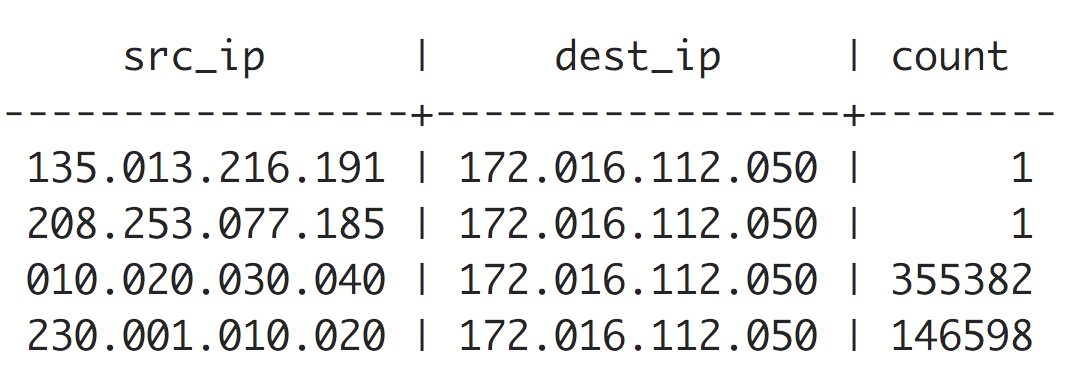
\includegraphics[scale=0.45]{T4_DARPA_1stDenseBlock.png}
    \caption{Network attack "neptune" in DARPA TCP Dump}
    \label{fig:t4_neptune}
\end{figure}


While for the \textit{Airforce TCP Dump} dataset, the attack types are mostly "smurf", followed by "neptune"" as shown in Table \ref{tab:airforce_t4.2}. Specifically, the provided labels are not always consistent (i.e. the same connection can be labeled as both "benign" and a type of "attack"). In such situation, we mark all these connections as "conflict" and treat them as a type of attack.

\renewcommand{\arraystretch}{1.2}
\begin{table}[!ht]
\centering
\caption{Five dense blocks in AirForce TCP Dump}
\label{tab:airforce_t4.1}
\begin{tabular}{|c|p{3.5cm}|p{2cm}|p{3cm}|}
\hline
\textit{\textbf{Block\_index}} & \textit{\textbf{Size}} & \textit{\textbf{Mass}} & \textit{\textbf{Density}} \\ \hline
{0}    & 1x1x1x2x1x1x1                & 2263941                              & 1980948.375           \\ \hline
{1}    & 1x1x1x1x1x1x1                & 263295                               & 263295.0              \\ \hline
{2}    & 1x3x3x2x1x53x25              & 431370                               & 34313.5227273        \\ \hline
{3}    & 1x2x2x1x1x79x20              & 420018                               & 27737.0377358        \\ \hline
{4}    & 1x1x1x2x1x2x2                & 52449                                & 36714.3             \\ \hline
\end{tabular}
\end{table}

\renewcommand{\arraystretch}{1.2}
\begin{table}[!ht]
\centering
\caption{Detected connection types in AirForce TCP Dump}
\label{tab:airforce_t4.2}
\begin{tabular}{|c|p{11cm}|p{2cm}|}
\hline
\textit{\textbf{Block\_index}} & \textit{\textbf{Connection Types}}  & \textit{\textbf{Total}} \\ \hline
{0}    & {'smurf.': 2263941}                & 2263941                               \\ \hline
{1}    & {'smurf.': 263295}                 & 263295                                \\ \hline
{2}    & {'portsweep.': 4, 'neptune.': 347786, 'benign': 12715, 'ipsweep.': 1, 'satan.': 10398, 'warezclient.': 1, 'conflict': 60465}                 & 431370                             \\ \hline
{3}    & {'satan.': 13, 'conflict': 9773, 'neptune.': 410232}            & 420018    \\ \hline
{4}    & {'smurf.': 52449}                 & 52449                                   \\ \hline
\end{tabular}
\end{table}

To better visualize the result, we draw the ROC curve (Figure \ref{fig:t4.3_roc} with the number of dense blocks varying from 1 to 20. Note that in the previous discussion, we treat those connections with inconsistent labels as network attack. Thus the result may vary from the others given different approaches of dealing with conflicting labels. 

\begin{figure}[!ht]
    \centering
    \subfigure{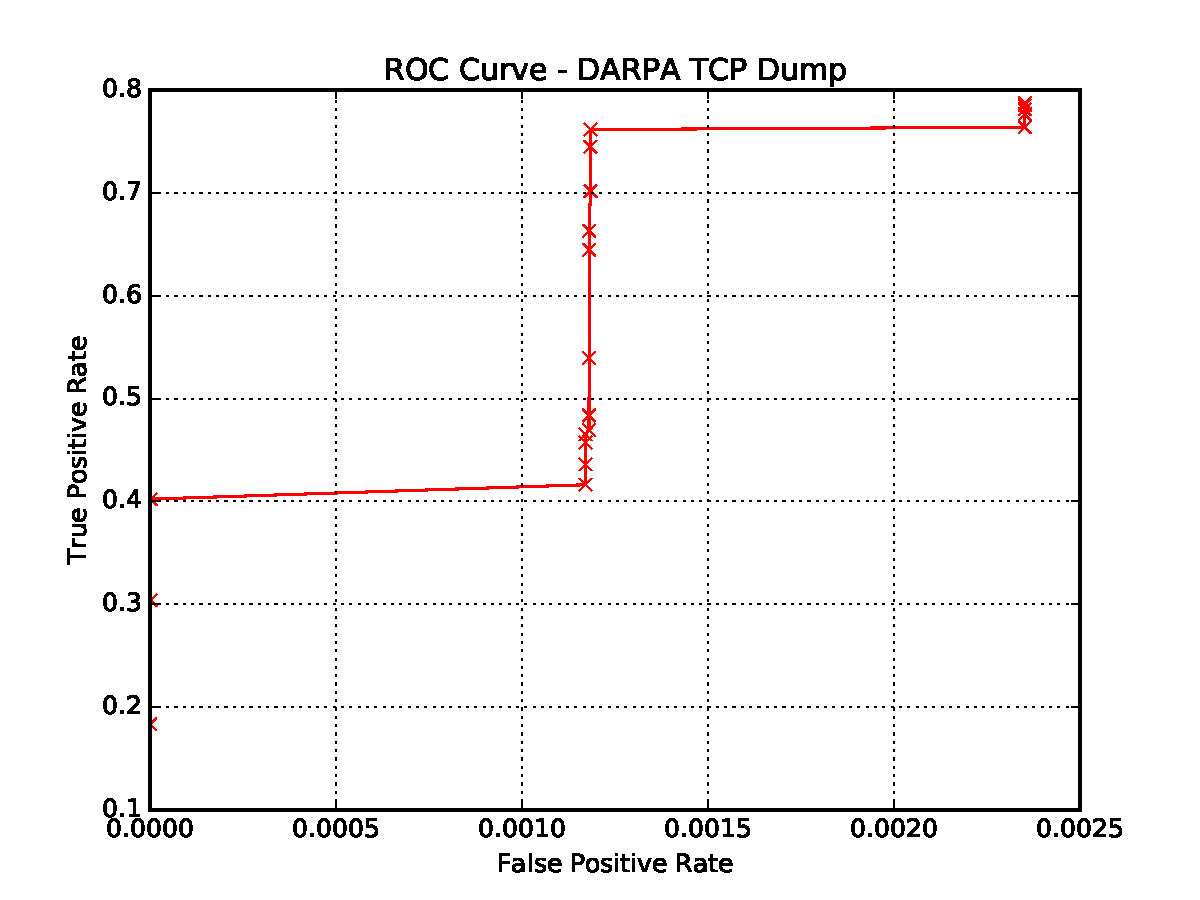
\includegraphics[scale=0.38]{ROC_Curve_DARPA_TCP_Dump.pdf}}
    \subfigure{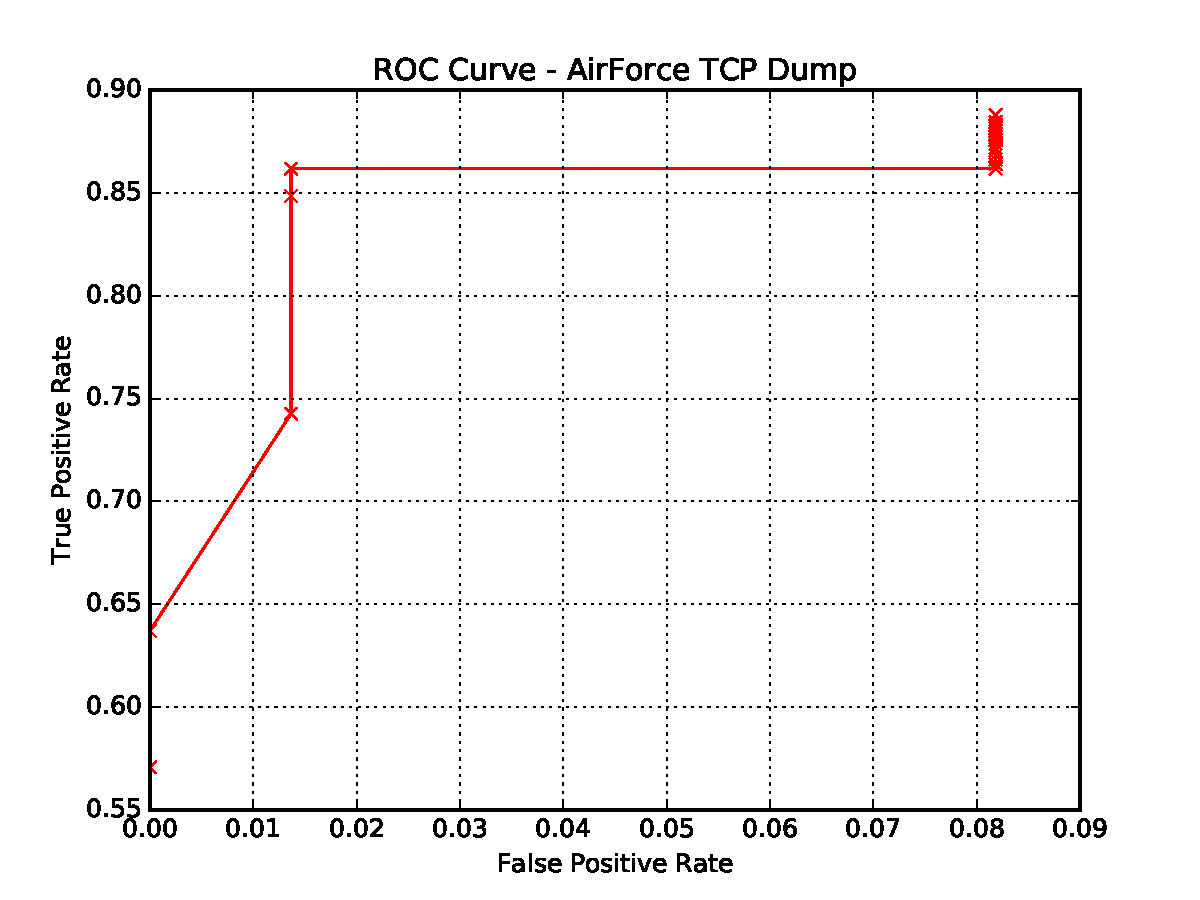
\includegraphics[scale=0.38]{ROC_Curve_AirForce_TCP_Dump.pdf}}
    \caption{ROC Curve - (a) DARPA TCP Dump (b) AirForce TCP Dump}
    \label{fig:t4.3_roc}
\end{figure}

With the statistics provided by the ROC curve, we compute the corresponding accuracy (AUC) using linear interpolation between data points and present them in Figure \ref{fig:t4.3_auc}.

\begin{figure}[!ht]
    \centering
    % \subfloat[]{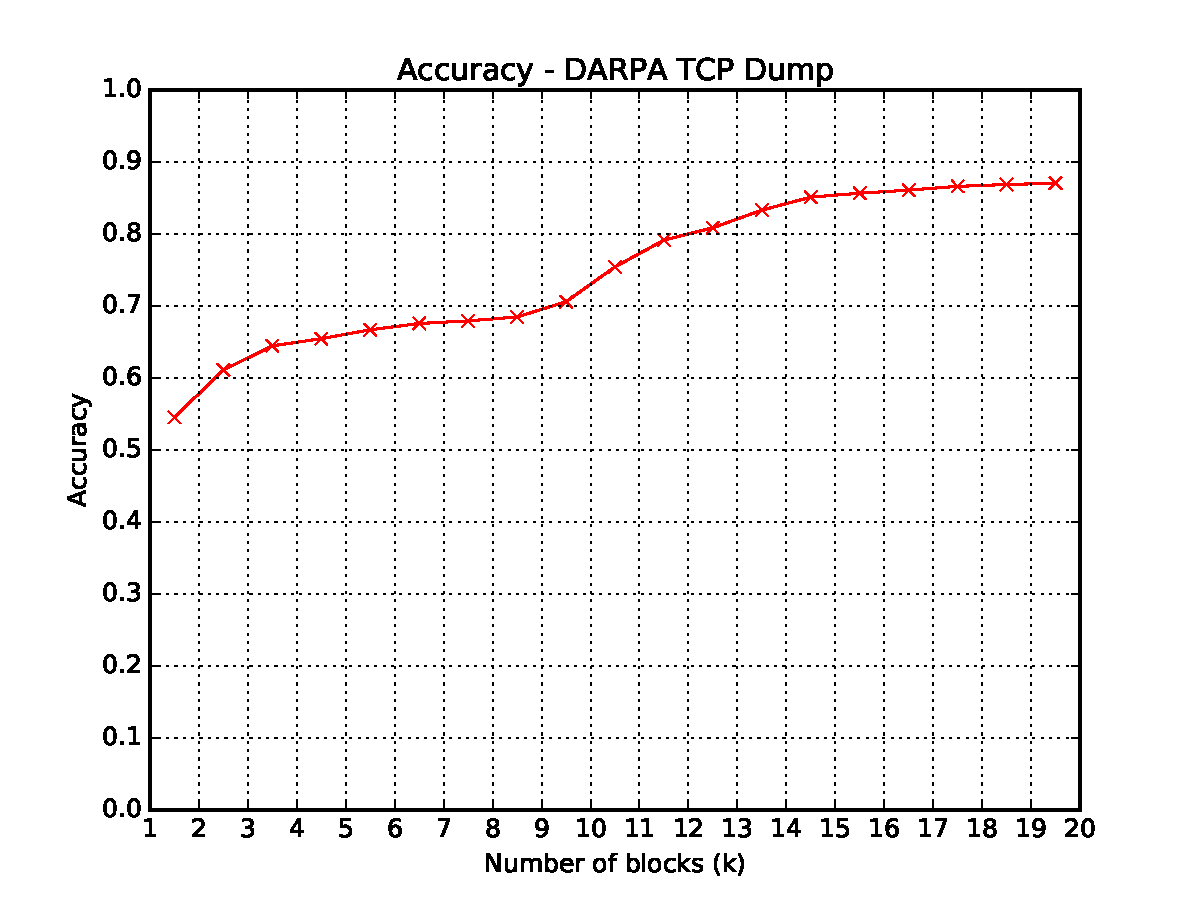
\includegraphics[scale=0.38]{Acuuracy_DARPA_TCP_Dump.pdf}}
    % \subfloat[]{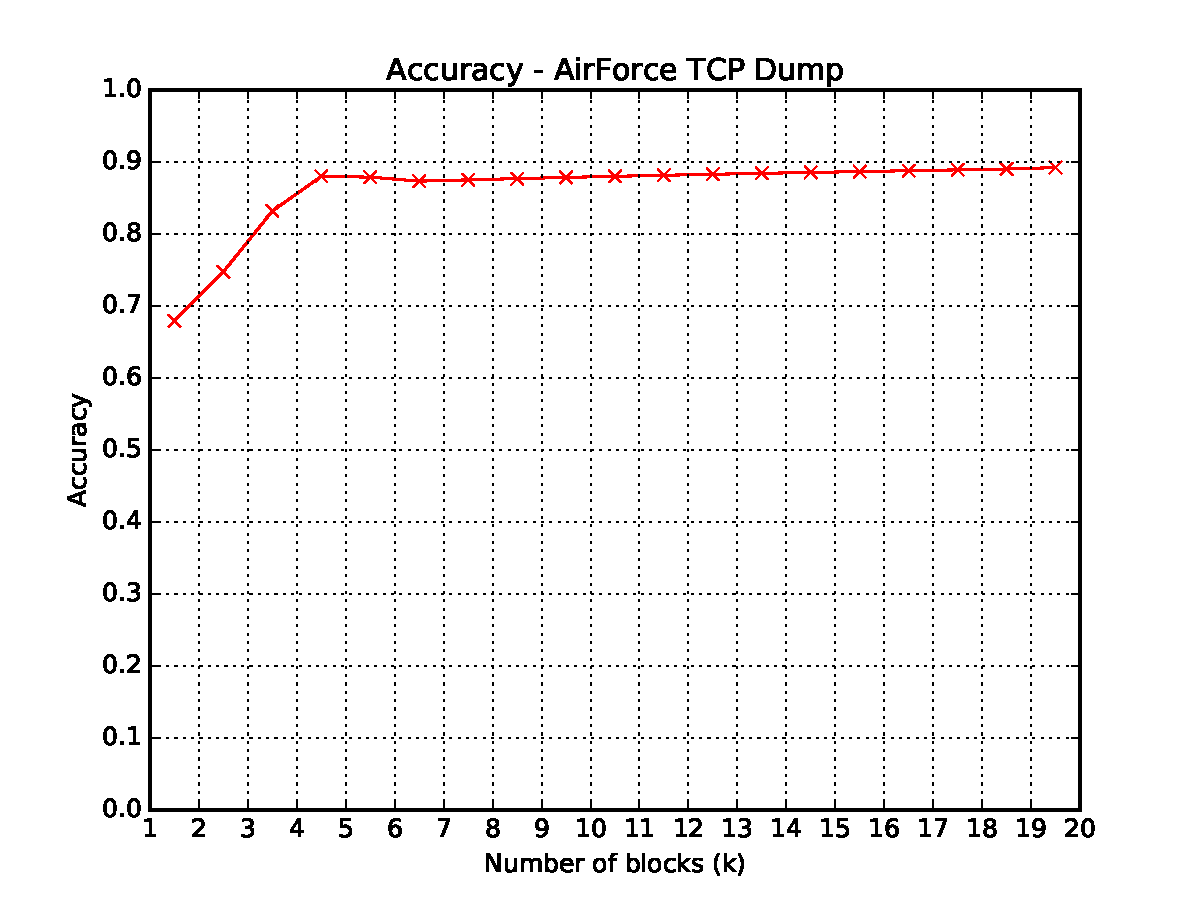
\includegraphics[scale=0.38]{Acuuracy_AirForce_TCP_Dump.pdf}}
    \subfigure{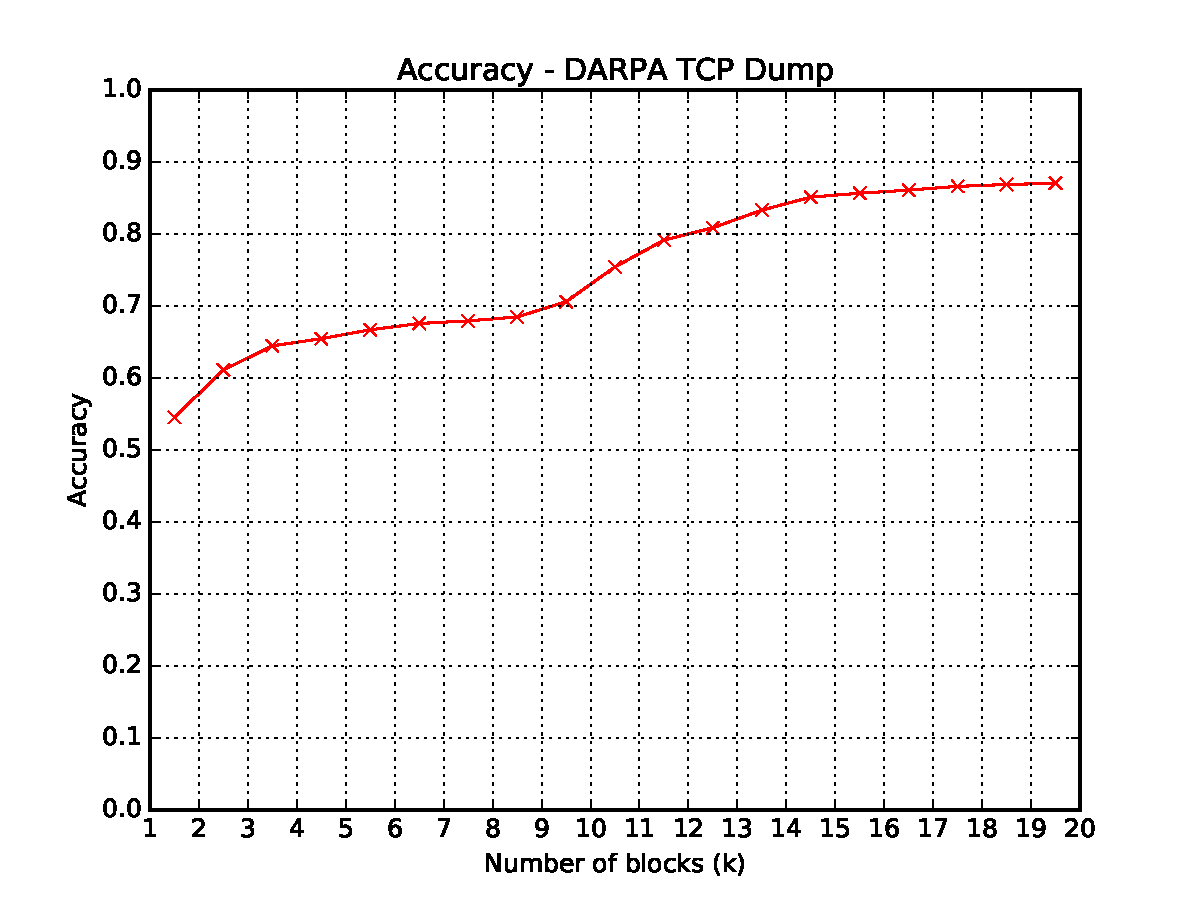
\includegraphics[scale=0.38]{Acuuracy_DARPA_TCP_Dump.pdf}}
    \subfigure{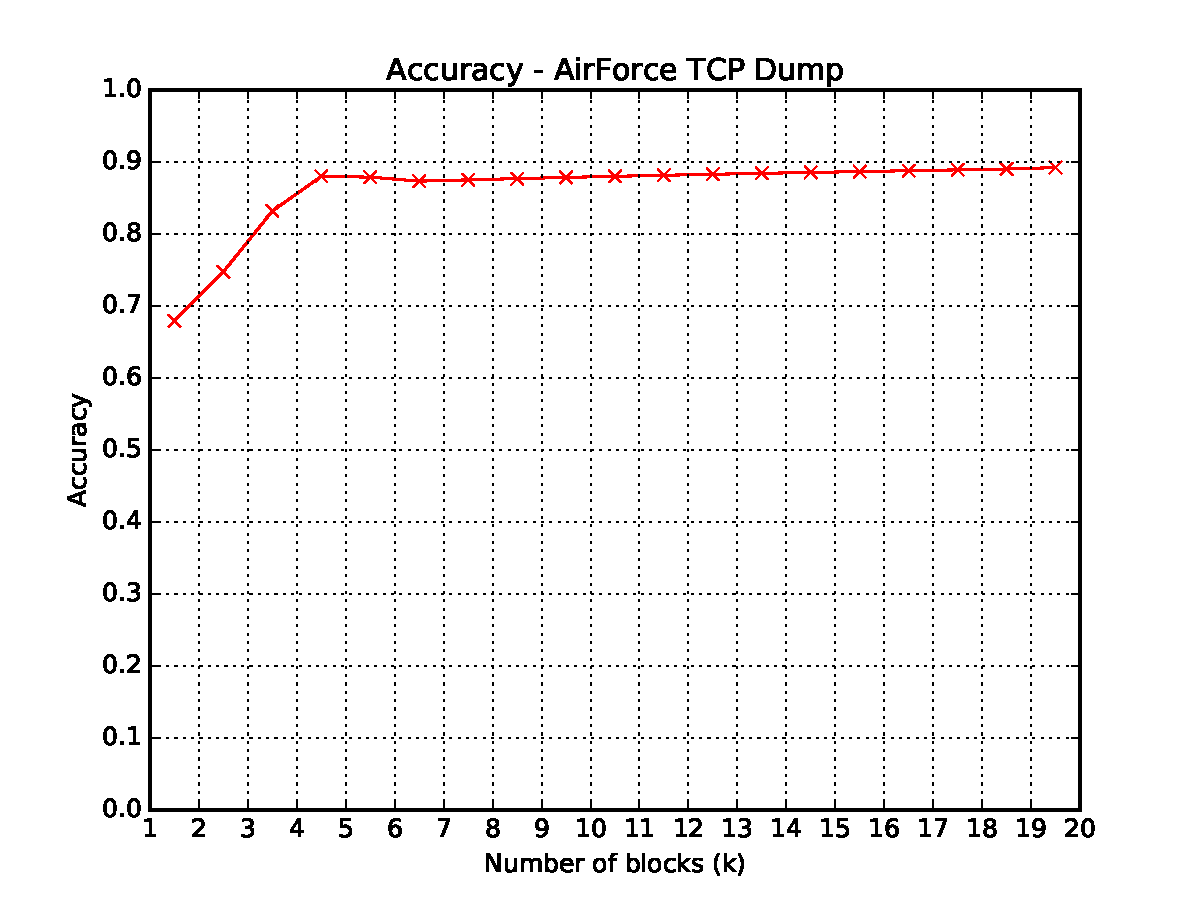
\includegraphics[scale=0.38]{Acuuracy_AirForce_TCP_Dump.pdf}}
    \caption{Accuracy - (a) DARPA TCP Dump (b) AirForce TCP Dump}
    \label{fig:t4.3_auc}
\end{figure}


\subsection{Anomaly Detection in Real-world Data (T5)}

We applied the D-Cube algorithm to multi-aspect datasets derived from the real world and analyze its performance by inspecting the related statistics of the detected dense blocks. Moreover, we dug into the retrieved records in the dense blocks and provide our justification on whether the detected dense blocks indicate anomalies or not. 

\subsubsection{Amazon Rating Dataset}

Table \ref{tab:amazon} presents the statistics of the first five detected dense blocks in \textit{Amazon Ratings} with $\rho=\rho_{ari}$, $k=5$ and Maximum density policy.  

\renewcommand{\arraystretch}{1.5}
\begin{table}[!ht]
\centering
\caption{Five dense blocks in Amazon Rating Dataset}
\label{tab:amazon}
\begin{tabular}{|c|p{4cm}|p{2cm}|p{3cm}|}
\hline
\textit{\textbf{Block\_index}} & \textit{\textbf{Size}} & \textit{\textbf{Mass}} & \textit{\textbf{Density}} \\ \hline
{0}                     & 60x60x1x1                 & 3600                               & 118.032786                           \\ \hline
{1}                     & 150x150x3x2                 & 7550                               & 99.016393                          \\ \hline
{2}                     & 40x40x1x1                 & 1600                               & 78.048780                           \\ \hline
{3}                     & 35x35x1x1                  & 1225                                & 68.055555                           \\ \hline
{4}                     & 3412x1745x1011x5                 & 77694                                & 50.344403                           \\ \hline
\end{tabular}
\end{table}

\subsubsection{Yelp Rating Dataset}

Table \ref{tab:yelp} presents the statistics of the first five detected dense blocks in \textit{Yelp} Ratings with $\rho=\rho_{ari}$, $k=5$ and Maximum density policy.  


\renewcommand{\arraystretch}{1.5}
\begin{table}[!ht]
\centering
\caption{Five dense blocks in Yelp Rating Dataset}
\label{tab:yelp}
\begin{tabular}{|c|p{4cm}|p{2cm}|p{3cm}|}
\hline
\textit{\textbf{Block\_index}} & \textit{\textbf{Size}} & \textit{\textbf{Mass}} & \textit{\textbf{Density}} \\ \hline
{0}                     & 60x60x1x1                 & 3600                               & 118.032786                           \\ \hline
{1}                     & 55x55x1x1                 & 3025                               & 108.035714                           \\ \hline
{2}                     & 50x50x1x1                 & 2500                               & 98.039215                           \\ \hline
{3}                     & 45x45x1x1                  & 2025                                & 88.043478                           \\ \hline
{4}                     & 5416x4464x2792x5                 & 268578                                & 84.744971                           \\ \hline
\end{tabular}
\end{table}



\subsubsection{English Wikipedia Revision History}

Table \ref{tab:wikipedia} presents the statistics of the first five detected dense blocks in \textit{English Wikipedia Revision History} with $\rho=\rho_{geo}$, $k=5$ and Maximum density policy.  



\renewcommand{\arraystretch}{1.4}
\begin{table}[!ht]
\centering
\caption{Five dense blocks in English Wikipedia Revision History}
\label{tab:wikipedia}
\begin{tabular}{|c|p{2cm}|p{2cm}|p{3cm}|}
\hline
\textit{\textbf{Block\_index}} & \textit{\textbf{Size}} & \textit{\textbf{Mass}} & \textit{\textbf{Density}} \\ \hline
{0}                     & 1x1x30                 & 7756                               & 2496.111889                           \\ \hline
{1}                     & 1x1x743                 & 8224                               & 908.002052                           \\ \hline
{2}                     & 1676x1x59                 & 30607                               & 661.879232                          \\ \hline
{3}                     & 1572x14x32                  & 1604                                & 18.028551                           \\ \hline
{4}                     & 2915x1x3                 & 2931                              & 142.264283                           \\ \hline
\end{tabular}
\end{table}
